%% 
%% Copyright 2007-2019 Elsevier Ltd
%% 
%% This file is part of the 'Elsarticle Bundle'.
%% ---------------------------------------------
%% 
%% It may be distributed under the conditions of the LaTeX Project Public
%% License, either version 1.2 of this license or (at your option) any
%% later version.  The latest version of this license is in
%%    http://www.latex-project.org/lppl.txt
%% and version 1.2 or later is part of all distributions of LaTeX
%% version 1999/12/01 or later.
%% 
%% The list of all files belonging to the 'Elsarticle Bundle' is
%% given in the file `manifest.txt'.
%% 
%% Template article for Elsevier's document class `elsarticle'
%% with harvard style bibliographic references

% \documentclass[preprint,12pt,authoryear]{elsarticle}

%% Use the option review to obtain double line spacing
\documentclass[authoryear,preprint,review,12pt]{elsarticle}

%% Use the options 1p,twocolumn; 3p; 3p,twocolumn; 5p; or 5p,twocolumn
%% for a journal layout:
%% \documentclass[final,1p,times,authoryear]{elsarticle}
%% \documentclass[final,1p,times,twocolumn,authoryear]{elsarticle}
%% \documentclass[final,3p,times,authoryear]{elsarticle}
%% \documentclass[final,3p,times,twocolumn,authoryear]{elsarticle}
%% \documentclass[final,5p,times,authoryear]{elsarticle}
%% \documentclass[final,5p,times,twocolumn,authoryear]{elsarticle}

%% For including figures, graphicx.sty has been loaded in
%% elsarticle.cls. If you prefer to use the old commands
%% please give \usepackage{epsfig}

%% The amssymb package provides various useful mathematical symbols
\usepackage{amssymb}
%% The amsthm package provides extended theorem environments
%% \usepackage{amsthm}

%% The lineno packages adds line numbers. Start line numbering with
%% \begin{linenumbers}, end it with \end{linenumbers}. Or switch it on
%% for the whole article with \linenumbers.
\usepackage{lineno}
\usepackage[dvipsnames]{xcolor}
\usepackage[capitalize]{cleveref}
\usepackage[inline]{enumitem}
\usepackage{siunitx}

\journal{Computers and Electronics in Agriculture}

\bibliographystyle{model2-names}\biboptions{authoryear}

\begin{document}

\begin{frontmatter}

%% Title, authors and addresses

%% use the tnoteref command within \title for footnotes;
%% use the tnotetext command for theassociated footnote;
%% use the fnref command within \author or \address for footnotes;
%% use the fntext command for theassociated footnote;
%% use the corref command within \author for corresponding author footnotes;
%% use the cortext command for theassociated footnote;
%% use the ead command for the email address,
%% and the form \ead[url] for the home page:
%% \title{Title\tnoteref{label1}}
%% \tnotetext[label1]{}
%% \author{Name\corref{cor1}\fnref{label2}}
%% \ead{email address}
%% \ead[url]{home page}
%% \fntext[label2]{}
%% \cortext[cor1]{}
%% \address{Address\fnref{label3}}
%% \fntext[label3]{}

\title{weatherprog N1 publishing quality-controlled data from heterogeneous stations}
%\title{}

%% use optional labels to link authors explicitly to addresses:
%% \author[label1,label2]{}
%% \address[label1]{}
%% \address[label2]{}

%\author{}
\author[dia]{Giuliano Langella\corref{cor}}
\address[dia]{Department of Agriculture, University of Naples Federico II, Via Università 100, 80055 Portici, NA, Italy}
\cortext[cor]{Corresponding author}
\ead{glangella@unina.it}

\author[deeit]{Raffaele Martino}
\author[deeit]{Massimo Nicolazzo}
\address[deeit]{Department of Electrical Engineering and Information Technology, University of Naples Federico II, Via Claudio 21, 80125 Naples, NA, Italy}

\date{February 2019}

\begin{abstract}
[COPIED] The current agrometereological monitoring of the Campania Region is both inadequate for its users and insufficient to support the simulation of pest risk models.
This work describes a cyber-physical system which has been designed to overcome these limitations, with the objective of
	\begin{enumerate*}
		\item automate all the tasks involved in climatic data management, including also the intervention of the human expert when appropriate,
		\item develop dependable pest risk models and provide the input data they need, and 
		\item provide real-time agrometereological data presentation.
	\end{enumerate*}
	The system is built around an automatic climatic data management engine called WeatherProg, which manages data collection, quality control, data reconstruction, and digital maps production.
	A proper climatic database has been developed to support the operations of WeatherProg, as well as a Web application for real-time publication of data handled by the software.
	Pest risk models, fed by point measurements and the digital maps produced by WeatherProg, are going to be prototyped.
	Furthermore, a new small measurement station has been prototyped, with the aim of being low-cost and easy to relocate, in order to support the characterisation and models parameterisation for different areas.
	This paper illustrates the current status of the system and discusses future directions.
\end{abstract}

\begin{keyword}
%% keywords here, in the form: keyword \sep keyword

%% PACS codes here, in the form: \PACS code \sep code

%% MSC codes here, in the form: \MSC code \sep code
%% or \MSC[2008] code \sep code (2000 is the default)

\end{keyword}

\end{frontmatter}

\linenumbers

%% main text
%\section{}\label{}
\section{Introduction}

%journal: Computers and Electronics in Agriculture
% https://www.journals.elsevier.com/computers-and-electronics-in-agriculture

% ==== Big Picture ====
%Include the big picture: The Earth Critical Zone requires that models such as SPA and pest models have quality checked data.
%\begin{itemize} 
%    \item Problem statement
%    \item Related work
%    \item Objectives
%\end{itemize}

% ==== Earth Critical Zone ====
%It is a living, breathing, constantly evolving boundary layer where rock, soil, water, air, and living organisms interact. These complex interactions regulate the natural habitat and determine the availability of life-sustaining resources, including our food production and water quality.
%The Critical Zone (CZ) is the support system for all terrestrial ecosystems, extending from unweathered rock to the top of any vegetation canopy. In the CZ, physical, biological, geological and hydrological processes interact at multiple temporal and spatial scales.
%Earth's critical zone is the “heterogeneous, near surface environment in which complex interactions involving rock, soil, water, air, and living organisms regulate the natural habitat and determine the availability of life-sustaining resources”
Climate controls the Earth's Critical Zone (ECZ) in combination with other physical, biological and geological processes.
The ECZ is a heterogeneous system extending from the top of the vegetation canopy to the bottom of unweathered rocks, regulates the availability of resources and modulates the production of ecosystem services such as the filtration and quality of water, and the production of food and fibre.

% ==== Agricultural Meteorology ====
% LINKS:
%   https://books.google.it/books?id=vdFBDwAAQBAJ&pg=PA22&lpg=PA22&dq=importance+of+agrometeo+measurements&source=bl&ots=CmcFAArYyq&sig=ACfU3U1TMqCpGqAv7VZjSz1M_IgPKv1--w&hl=it&sa=X&ved=2ahUKEwjPs_Tdg_vgAhXQ4KQKHYM3B4AQ6AEwAHoECAkQAQ#v=onepage&q=importance%20of%20agrometeo%20measurements&f=false
%   http://www.agrometeorology.org/files-folder/repository/gamp1.pdf
%   https://en.wikibooks.org/wiki/Introductory_Agrometeorology/Introduction
%   http://www.agrilearner.com/agrometeorology-needs-scope/
%   http://www.agriinfo.in/default.aspx?page=topic&superid=1&topicid=377

%Weather: Physical state of the atmosphere at a given place and given time. Eg. Cloudy day
%Climate: Long term regime of atmospheric variables of a given place or area. Eg. Cold season
%and considered as basic input or resources in agricultural planning, every plant process related with growth development and yield of a crop is affected by weather.

Weather and climate are the most important dynamic components of the ECZ determining the physical condition in which animals and plants are grown.
Agricultural meteorology is concerned with the monitoring of weather and the characterisation of the meteorological, hydrological and pedological factors that have a direct effect on agriculture and the production of crop and livestocks.
% http://www.agriinfo.in/default.aspx?page=topic&superid=1&topicid=377
Agricultural meteorology is deemed important considering the large amount of ground stations available worldwide to monitor the behaviour of weather elements, notwithstanding, for instance, the huge amounts of air-borne proxy products coming from a massive satellite monitoring.
Indeed, it helps (search one or more REFs for each item): 
    \begin{enumerate*}
        \item understanding the realisation of several crop parameters such as the growing season and the harvesting time;
        \item managing crops by means of various farm operations such as fertilisers application and irrigation scheduling;
        \item assessing the suitability of specific crops in space (by means of agroclimatic zoning) and time (e.g. according to climate change);
        \item crop and livestock monitoring and modelling;
        \item understanding the spatial distribution of soils types and properties since climate is one of the soil forming factors recognized in the CLORPT (REF: Jenny) or SCORPAN (REF: MacBratney) models;
        \item forecasting plant pests and diseases.
    \end{enumerate*}

Therefore there is an increasing demand for the production of digital climatic data of good quality within the earth critical zone both 
    for practical applications (e.g. the need to know climatic patterns in a farm to improve the management),
    and
    for research and development, in particular to simulate the soil-plant-atmosphere system and the risk of pests.
The demand is particularly burdensome considering the requirement to handle climatic data both at finer temporal scale and in a continuous spatial domain.
It means that daily (e.g. in the soil hydrological modelling) or even hourly records (e.g. in the phytopathologic risk modelling) measured at point gauges sparsely located in a territory must be transformed in three dimensional climatic data cubes (Longitude, Latitude, Time) by means of statistically sound geospatial procedures.
% (there is a gap between the major of scientific modelling approaches that requires digital climate maps and the gauged measurements).
There exist few approaches implementing and deploying automatic spatial inference engines of this kind based on point climatic data at the daily or even at the hourly time step.
One example working in USA with daily data, is given by the expert-based model called PRISM developed by  \cite{Daly08_PRISM_USA}. (\ldots search for other REFs.)

% ==== Aim ====
%Support systems to agrometeorological practices and services comprise data (so quantification), research, training/education/extension and policy environments. Especially in industrialized countries mathematical models are increasingly used in operational agricultural meteorology, in conjunction with Geographic Information Systems (GISs) to provide inputs to Decision Support Systems (DSSs).
Especially in more developed countries, mathematical models are increasingly used in agriculture in conjunction with Geographic Information Systems (GISs), also via web in the form of WebGIS, to provide inputs to Decision Support Systems (DSSs), possibly via web in the form of Web Based geoSpatial Decision Support Systems (WB-SDSS).

\ldots there is a huge production of DSS on quite every aspect of the agricultural or forestry systems \ldots

In this paper a strongly modular Geospatial Cyber-Infrastructure (GCI), called MyNameIsBeautiful, is proposed as a general technological framework being a WB-SDSS, that can be fully tailored to the specific needs of an existent agrometeorological network.
The proposed GCI is based on a software component, namely WeatherProg \citep{langella:weatherprog2014,langella:weatherprog2016}, which represents the main engine of the information technology system and has the potential of being the basic engine of whatever geospatial-based service in agriculture, in which both the weather and the climatic information is of paramount importance.
WeatherProg has the key advantage of implementing all the tasks from gathering the raw measurements coming from the agrometeorological sensors till the delivery of digital climatic maps at both daily and hourly time steps.

Together with the presentation of the general template WB-SDSS, the results of applying the MyNameIsBeautiful GCI to a specific case study, that is in Campania Region, is shown with the specific focus of producing data of good quality.
The task consists in tuning a fully automatic or assisted procedure to quality check the measurements at the gauged points.
This is of particular relevance given on one hand some limitations, such as the eco-environmental complexity of the study area, the scarcity of stations and the lack of long term time series for any station, and on the other hand the urgent need for monitoring and sharing agrometeorological data (highlight the important step forward thanks to our GCI) and the urgent need for a system to assist the production of bulletins to help mitigate the effects of alien or autochthonous pests.
[ENHANCE!] The need for tools than can enhance the climatic data distribution, improving environment/farm management; this implies that in Italy (and also find the EU regulation and apply the discourse to EU itself) PAN advises administrative units in charge of agrometeorological publication to provide climatic data but also pests bulletins (by using possibly mechanistic modelling) based on climatic data which are able to support decision making at the farm level, with the result of decreasing the amount of pesticides with the twofold effect of reducing costs and diminishing environmental impact of by-products.

\section{Materials}

\begin{figure}
	\centering
	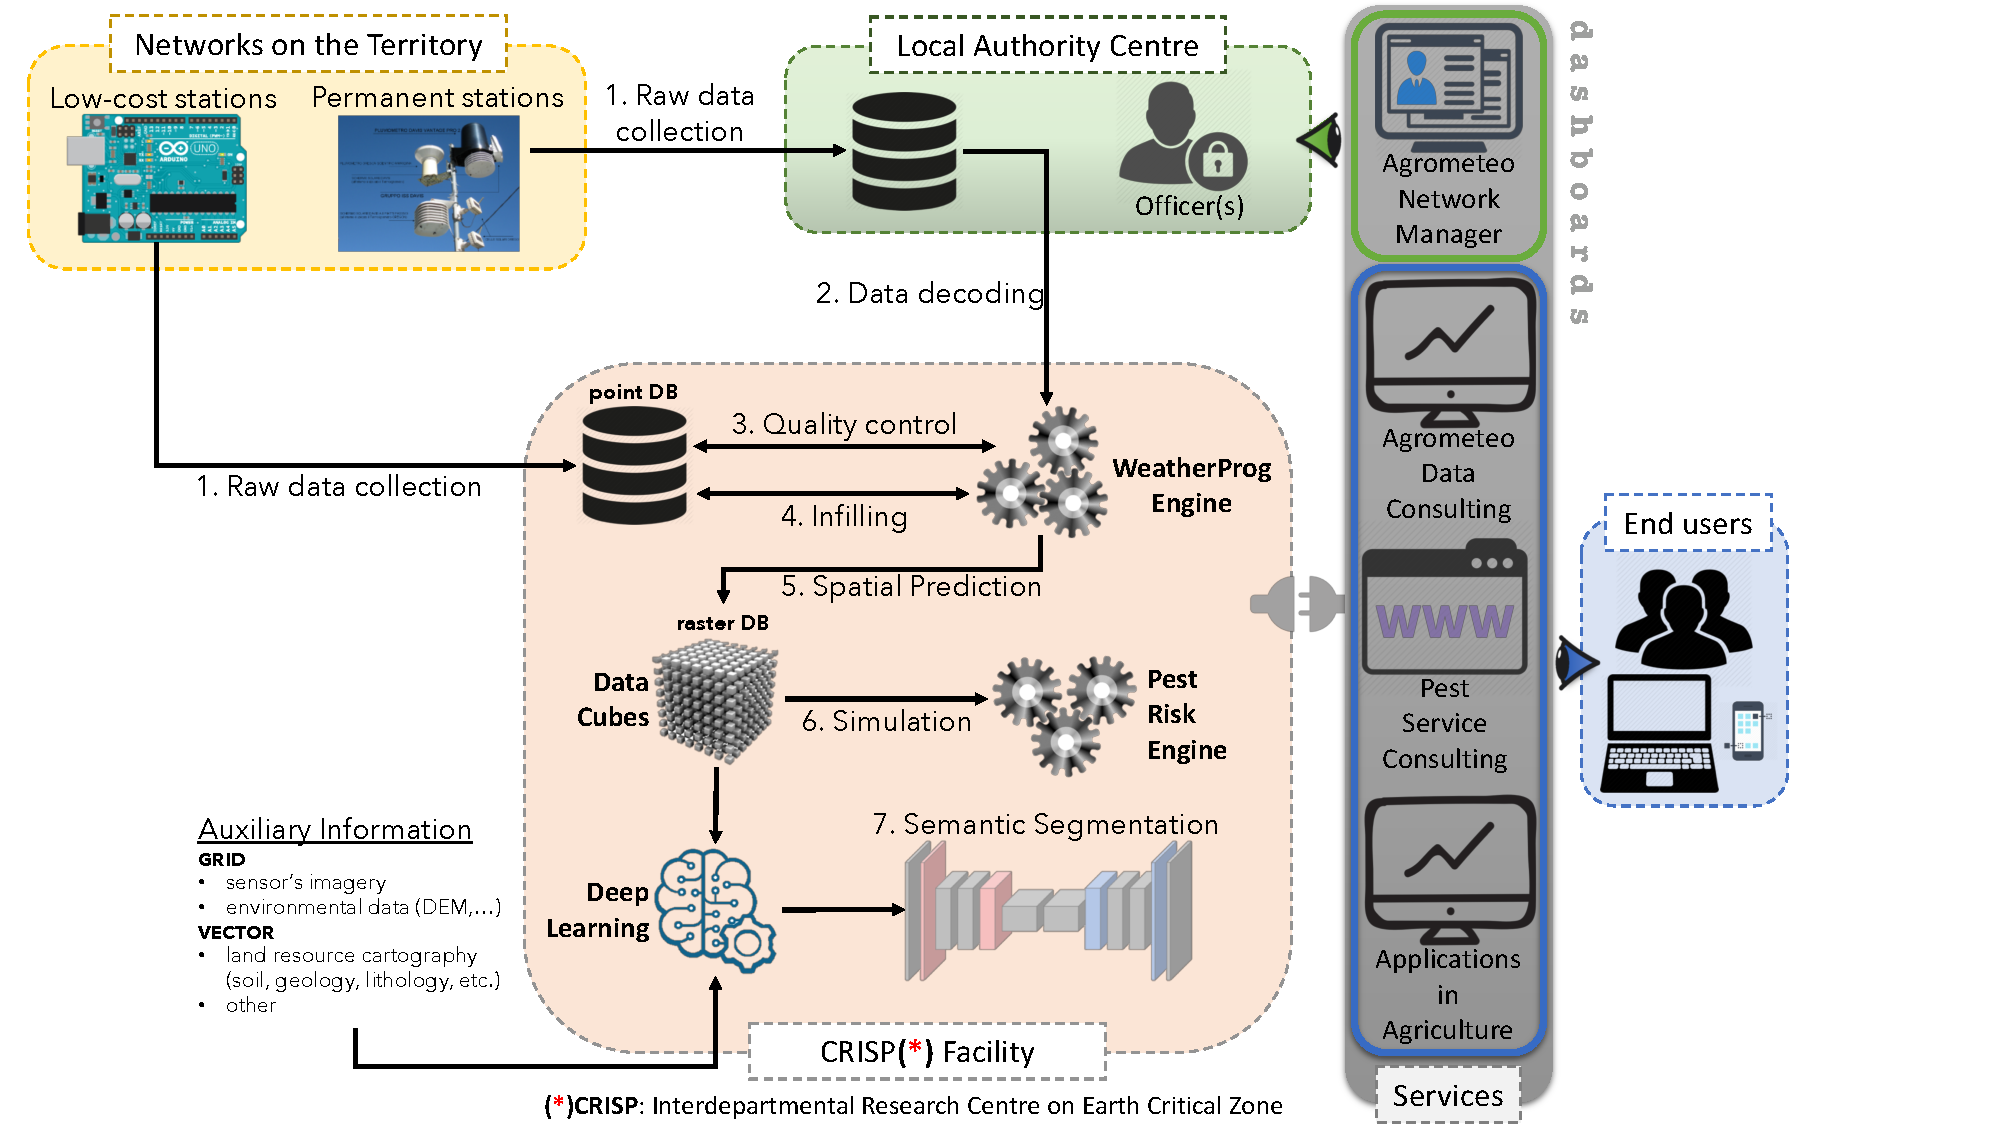
\includegraphics[scale=.5]{figures/fullSystem_GCI.pdf}
	\caption{High level architecture of the proposed cyber-physical system}
	\label{cyberPhysicalSystemFig}
\end{figure}

\subsection{Study area}
[COPIED] Located in southern Italy between \ang{13;45;}E, \ang{15;49;}E, \ang{39;59;}N and \ang{41;31;}N, Campania is the third most populated region of the country, but due to its extension of about \SI{13600}{\metre\squared}, it is the most densely populated region of Italy.
Its inland is occupied by the Apennine Mountains, oriented roughly NW-SE, whereas the Sele and Campana plains border the coast.
The Sele plain is named after the river which traverse it, while the Campana plan is traversed by the Volturno river.
Nevertheless, the majority of the regional territory is hilly, for the 50\% of the territory, against the 35\% mountainous and the 15\% flat.
Consequently, the elevation ranges from \SIrange{0}{1904}{\metre} above mean sea level.

    It covers an area of about 13,600 km2, and is the third most populated region in Italy.
    AGRONOMIC INFO\dots e.g. the production of products of particular quality (DOP, IGP, DOC, DOCG; \dots)\\
    AGRO-ECONOMY\dots e.g. the ecomic value of the regional production in the primary sector\\
    Physiographic analysis: La Campania è prevalentemente collinare (50.8\%), il 34.6\% di essa è montuosa e il 14.6\% pianeggiante\\
    
    Morphologically, Campania has a complex terrain: the Apennine Mountains in its eastern sector are oriented roughly NW–SE, while the coastal plains of Campana and Sele occupy its west, traversed by the Volturno and Sele Rivers respectively.
    The Campana plain, developed in subsiding grabens, is infilled by abundant sediments originating from Apennine chain erosion and the products of intense volcanic activity.
    In addition to sedimentary rocks (limestone, siliceous schist and terrigenous sediments), the plain contains volcanic rocks (potassic/ultrapotassic lavas and pyroclastics) from Roccamonfina, Somma–Vesuvius Mts., Campi Flegrei and Ischia.
    Elevation range from zero to 1904 m above mean sea level.
    Agrometeorologial stations are located from XXX m to YYY m above mean surface level.
    %A second study area is Cilento, a geographical district of about 6000 km2 in southern Campania delimited by the Sele plain to the north. It consists mainly of hills in stratified flysch (Alento wa- tershed) and limestone reliefs (Mt. Alburno, Mt. Cervati, etc.).
    %Its landscapes also include marine landforms.
    %This area is characterized by a very sparse rain gauge network, and was selected specifically to evaluate the performance of the bootstrapping technique on a more limited dataset.

\subsection{The cyber-physical infrastructure}

Central to the design of an effective automated data-processing system is the database. The telecommunications subsystem database must hold:
(a) Bulletins of incoming messages;
(b) Locally generated observations;
(c) Products for national dissemination;
(d) Bulletins of locally generated observations for transmission on the GTS.
The applications subsystem database must hold:
(a) Reports derived from decoded bulletins;
(b) Fields derived from decoded bulletins;
(c) Products prepared through the processing of reports and fields.
If possible, the database residing in each computer should be controlled by the same database
management system (DBMS), which should be relatively simple so as to minimize computing overheads and facil- itate the speed of response of the overall data-processing system.
    
\subsubsection{Official agrometereological network (RAR) monitoring}\label{RARStructure}
The agrometereological monitoring is in charge of the Agrometereological Regional Centre (CAR) under the Department for Agriculture of the Campania Region. The station network run by the CAR includes, at the time of this writing, 34 stations spanning an elevation range from \SIrange{11}{794}{\metre} a.m.s.l.

Not only the number of available stations is too limited to properly capture the aforementioned complexity of the regional environment, but also the equipment of these stations is highly variable.
All the stations measure air temperature, rainfall and air humidity, but for 10 stations these are the only climatic parameters measured.
Air pressure is measured by only 9 stations.
All the 11 fundamental climatic variables are measured by at least one station in the network, but no one station is equipped to measure all the climatic variables.

\begin{itemize}
    \item The current net inadequately covers the complex territory of the Campania Region, in terms the representativeness over both elevation and geospatial domain.
    \item the current web application cannot adequately share the measurements according to the requirements of potential users (DELETE:coming form different "productivity" sectors, BETTER: stakeholders), such as agriculture, professionals in agronomy supporting the farmers, livestock farmers, etc.
\end{itemize}

It is a WMO-compliant monitoring net\\
Describe the RAR (description of station and db/server)\\
show a map with locations\\
present a table with a summary of sensors, duration of monitoring, and so on. \\
describe FTP setup


\subsubsection{Monitoring with Low-Cost Station (Massimo)}
It is a monitoring net using low-cost and open-source components.

\begin{itemize}
    \item Hardware components
    \begin{itemize}
        \item Base board
        \item Sensors
        \item Network chip
    \end{itemize}
    \item Firmware logic
\end{itemize}

\subsubsection{Weatherprog (Giuliano)}
[COPIED](start linking to soilconsweb but underline today implementation of WeatherProg to demonstrate its usefulness, powerfulness and readiness-of-use)\\
WeatherProg is a computer program that was developed as the baseline asynchronous engine for the raw weather records handling within the SOILCONS-WEB project (LIFE08 ENV/IT/000408, cite the papers by Langella, 2014 and Terribile et al., 2015)... 
It was developed because... 
This project ended in dec-2014, but (go to next sentence, explaining nowadays usage of WeatherProg).\\
WeatherProg is now used as a geospatial weather engine in a web-based DSS for on-the-fly and real-time (the time interval only depends upon the station data logger query frequence) consulting of agrometeorological variables... allowing temporal/spatial stats queries and embedding CUDA codes (on the client-side GUI) for fast calculation. Then also WeatherProg itself has major CUDA developments in order to speedup crucial and time-consuming calculations such that of making spatial interpolation at any pixel of the study area)\\


WeatherProg \citep{langella:weatherprog2014} is a computer program to automatically manage agrometeorological data.
The first implementation was carried out as the baseline asynchronous engine for the raw weather records handling in the SOILCONS-WEB project (LIFE08 ENV/IT/000408).
The program was progressively modified and updated in order to be accommodate the requirements of both (i) Regional Administrative Bodies in charge of data management and publication and bulletins production for pest management, and (ii) the setting of a service in the context of Agriculture 4.0 and advanced IoT.

Raw reports from a climatological network can be ingested as input and a different set of operations are performed ranging from the data checking to the delivery of gridded weather parameters.

Temperature, rainfall, relative humidity, solar radiation, atmospheric pressure and wind speed are the agrometeorological variables most commonly handled by the program using different temporal scales calculated by the aggregation of the most fundamental units of measurements, i.e. the 10-minute  measurements which are aggregated to build hourly and daily data.

WeatherProg starts automatically every hour when a new report is available, carrying out the following main operations:
\begin{enumerate}
    \item The real-time report with measurements from all sensors and stations belonging to a monitoring network arrives to WeatherProg via a secure file transfer protocol. [data retrieval]
    
    \item After the report is decoded according to time scale and sensors, data are ingested in PostgreSQL. [data decoding]

    \item Quality check of time series to automatically demarcate good measurements from wrong and missing values, which are conveniently flagged for the subsequent infilling procedure.
    An anomalous datum is detected thanks to a multilevel technology based on interlinked and different kinds of quality checks such as logical, climatologic, spatial, temporal and persistency checks. Certification of abnormality is semi-automatic and is the result of the combination of the data-driven WeatherProg checking procedure and the knowledge-based human checking in order to finally assign the definitive flag (such as GOOD, WRONG and so on).
    
    \item Anomalies and missing data are all flagged to be interpolated by means of an automatic linear regression procedure.
    Different methods of interpolations are available such as a deterministic method (based on moving average with growing kernel) or a statistical method (a stepwise multilinear regression using other stations after an optimization step). [data infilling]
    
    \item The spatial interpolation of point data is performed considering the scale of the application that is requesting WeatherProg to produce the digital maps.
    Three-dimensional climatic data cubes (easting, northing and time) are produced which allow queries along any of the dimension (such as slicing, dicing and trimming). The methods available for spatial interpolation are the IDW (parameterized inverse distance weithed), different flavors of kriging (ordinary, regressive), and a PRISM-like approach. [spatial interpolation].
\end{enumerate}

\subsubsection{IT-decode [Raffaele]}\label{decode}
To provide support for data storage, the PostgreSQL Data Base Management System (DBMS) \citep{postgres} has been chosen. PostgreSQL is the fastest relational DBMS, and is open-source; but the most relevant reason for its choice is its comprehensive support of spatial data. PostgreSQL features natively a number of geometric types and operators over them but, most importantly, it comes with an optional, open-source, extension named PostGIS for full support of geographic data. This extension is a cornerstone in our plan for future improvement of the automated system.

Theoretically, Weatherprog could directly access the PostgreSQL database, by embedding SQL queries into the code of its core modules. This approach would strictly couple Weatherprog with the database structure, with the considerable downside of requiring to modify each and every relevant query in the code when a change of the database structure is applied. To enhance modifiability, we chose to have a dedicated persistence module instead. This way, Weatherprog's core modules no longer need to know, and therefore depend upon, every detail of the database architecture, instead it makes meaningful calls to the functions made available by the persistence module. Technically speaking, the persistence module, which is developed taking advantage of the object-oriented features of the Matlab\textsuperscript{\circledR} language, effectively provides an \emph{Application Programming Interface} (API) for using by the other modules of Weatherprog. When a structural change is applied to the database, the modification to the Weatherprog code is concentrated and limited to the persistence module, without affecting the other modules.

 \paragraph{Decoding of incoming data} Data as received from CAR is not suitable to be inserted into the data base. Each record of the incoming table contains all the measurements of all the climatic variables of all the stations in the RAR; such a record would clearly be poor effective and poor efficient, pointlessly grouping in a single record unrelated data; not to mention that such a record would violate WMO prescriptions about proper handling of climatic data \citep{wcdmp:cdms}.
 
 More importantly, the incoming table labels measurement of the same climatic variable with different names, making any attempt of data analysis impossible. To make things worse, the format of the incoming table is subject to change. The most relevant task of the decoding module is to map the different names of the same climatic variable to a standardised attribute, which is also employed by the database.
 
 For performance reasons, the data insertion is performed with a single SQL INSERT statement per climatic variable. This means that, given the all-or-nothing behaviour of SQL statements, each record to be inserted must be valid, otherwise the whole insertion will fail. It is therefore Weatherprog's responsibility to ensure that all the data submitted to the database can actually be inserted.
 
 To this end, the decoding module checks whether the data to be inserted is already present, since the insertion of a duplicate record would be rejected by the database. These checks have been optimised in order to avoid an excessive overhead due to database access: each database query is highly time consuming, fairly regardless of the complexity of the query. For this reason, it is highly impractical to check the presence of each value independently, on the contrary more complex queries, with the capability of validating a larger share of the data to be inserted, have been developed.
 
As said earlier in \cref{RARStructure}, data is sent from CAR on an hourly basis,  containing all the measurements of the previous 24 hours. To handle the hourly dispatch and provide data to the end users as soon as they are available, the system is configured to automatically have a run of Weatherprog every hour, by means of the \texttt{cron} daemon of the Unix systems. This hourly run is in charge of updating the database with the data related to the last hour. Late updates of the incoming data are dealt with by another periodic run of Weatherprog, but on daily basis. This daily run works on the whole 24-hour incoming table, check which time ranges are missing within the database and fills them. \textcolor{Red}{It is useful to mention the daily run here, even if it has not been implemented yet}

\begin{figure}
	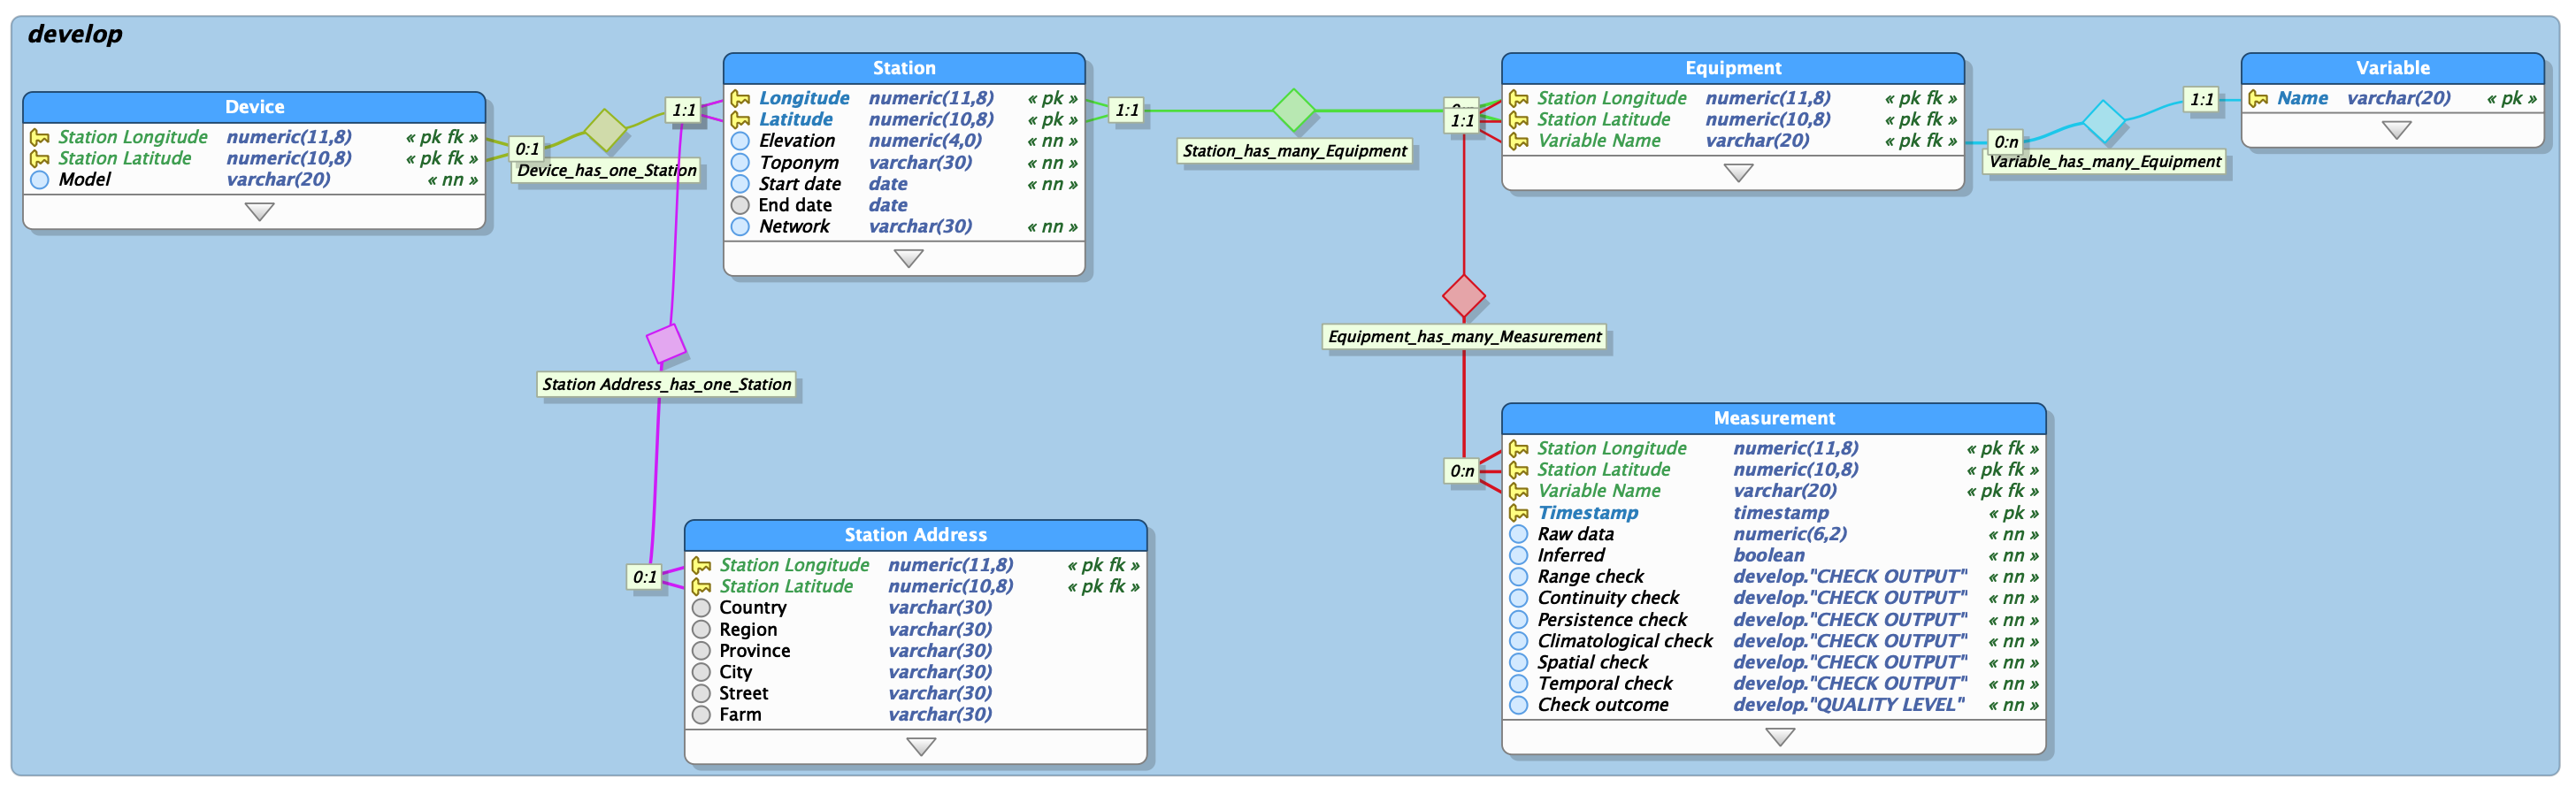
\includegraphics[scale=.26]{ERD}
	\caption{The data model for the climatic database. Each box represents a table. Each row in the box represents a field of the table. The yellow key denotes fields which form the Primary Key of the table. The blue circle denotes field which cannot be left empty by any record. Diamond-marked links means relationship within table subject to referential integrity constraints. Fields which are part of the Primary Key and subject to referential integrity constraints are written in green.}
	\label{ERD}
\end{figure}


\paragraph{Data model}\textcolor{Red}{Version 3.0, assuming that the merging of the climatic data has been carried out} The data model of the data base has been studied to help maintaining data consistency. Its design allows to avoid a number of unconsistencies thanks to the relational checks performed by the DBMS. 

The data model is illustrated in  \cref{ERD}, which illustrate the logic-level \emph{Entity-Relationship Diagram} (ERD), ready to be implemented in SQL automatically by means of the \emph{pgModeler} \citep{pgmodeler} open source software. For the reader unfamiliar with data modeling, the boxes representing tables of the database, with the fields listed within each box. The diamond-marked links represent a reference from a table to another subject to \emph{referential integrity constraints}, which are validity checks automatically performed by the DBMS. Further details of the model are described in the caption of \cref{ERD}.

Each measurement site is represented by an entry of the \texttt{Station} table. A station is uniquely identified by its coordinates. The toponym field is indispensable since it is employed, along with the station's elevation, by the web application to label the station itself. The date when the station was added to the network is recorded, as well as the withdrawal date for these stations which have been dismantled. The Network field provides support for the integration of different monitoring network, which is discussed in all its aspects in \cref{Integration}.

Additional pieces of information which may be available for the station are stored in separate tables. The advantage of this choice is twofold. Firstly, due to the fact that records are physically stored sequentially in the mass memory,  it is faster to access shorter records rather than having to "jump" unnecessary, often empty fields. Lastly, with this design there is no space allocated in the quite common case that these pieces of information are not available, contrarily to the need to waste space for empty columns. This splitting is profitable since data in the separate tables are not needed by the day-to-day operations of Weatherprog, and are only seldom used by the web application.

The table \texttt{Station Addresses} stores additional information about the location, most notably the farm whether the station is hosted. In fact, this data is more meaningful for the low-cost stations, and it is often not available for the permanent station. The table \texttt{Device} holds additional information about the rig which actually performs the measurements. Currently, only the model of the device is available.

The other fundamental table is the \texttt{Measurements} table. The measurements of all the climatic variables of all the stations are stored in this table. This choice has been made to allow coalescing of accesses, since it has been observed that it is faster to execute a single complex query rather than several simpler queries. More specifically, the controls required by the decoding module can be performed on all the variables simultaneously, and the insertion of new data can be performed with a single SQL statement. Each measurement is uniquely identified by the station which performed it, the climatic variable measured and the date and time of the measurement, and is accompanied by a series of flags, one for each control module, as described in \cref{controlFlags}. It is worth mentioning that, due to the choice of not to have a weird identifier of the stations, the coordinates of the station end up in the \texttt{Measurements} table. The availability of this piece of data allows for avoiding SQL JOINS to perform spatially-parameterized queries on the measurements. Constraints are defined to avoid any "structurally" invalid data.

The \texttt{Equipment} table lists all the climatic variables each station can measure. The fact that is this the referring table of the referential integrity constraint from the \texttt{Measurement} table ensure that a measurement for a variable that a station is not able to measure \textbf{cannot be inserted}, and this is verified directly by the DBMS.


\section{Methods}
\subsection{IT-qcheck [Raffaele] * 25-02-2019}\label{controlFlags}
The data storage provides support to the quality control procedures by storing, for each measurement record, one flag for each control module, and a flag for the overall result of the quality control.

Each of the flags for the quality control modules can assume one of the following values:
\begin{description}
	\item[UNPROCESSED] The measurement has not been subject to the quality control. \textcolor{Red}{This flag no longer makes sense with the addition of the overall quality control flag, and should not be mentioned if not removed altogether}
	\item[DISABLED] This quality control module was not enabled for this measurement
	\item[UNCHECKED] Quality control was performed on this measurement, but this specific quality control module has not been applied yet.
	\item[CORRECT] This measurement appears to be correct according to this quality control module.
	\item[DUBIOUS] This measurement is suspicious, according to this quality control module, which cannot decide either for correctness or for wrongness.
	\item[WRONG] This measurement appears to be wrong according to this quality control module.
	\item[MISSING] This measurement is not present in the database \textcolor{Red}{This flag no longer makes sense with the current version of the database, and should not be mentioned if not removed altogether}
	\item[INVERTED] This measurement of a maximum (minimum) value of a climatic variable appears to be inverted with its respective minimum {maximum} \textcolor{Red}{This flag no longer makes sense with the current version of the database, and should not be mentioned if not removed altogether}
\end{description}

On the other hand, for the overall quality control flag the following values are defined:
\begin{description}
	\item[UNPROCESSED] The measurement has not been subject to the quality control.
	\item[UNDECIDED] The measurement has been subject to some quality control modules, but the procedures have not ended yet.
	\item[WRONG] The measurement appears to be wrong, according to Weatherprog.
	\item[DUBIOUS] The quality control procedures cannot decide either for correctness or for wrongness. Manual intervention of an operator is required to estabilish the correctness of the measurement.
	\item[CORRECT] The measurement appears to be correct, according to Weatherprog.
\end{description} 

As said earlier in \cref{decode}, there are two periodic runs of Weatherprog in charge of the decoding task. These runs are also useful to perform quality control checks on different windows of data. \textcolor{red}{Details of which controls are executed when, to be provided}

\subsection{Automatic quality control (semi-automatic on demand) [Giuliano]}
The quality check reads data stored in a relational database (in our case PostgreSQL)[UP]\\
and applies a procedure based on a multi-step and variable-oriented procedure.

NOTES: (flags and meaning: UP)\\
logic of the checks;\\
kind of checks (range, logic, climatologic, temporal, spatial, ...)

\begin{itemize}
    \item qcheck m10, T + R
    \item qcheck h1,  T + R
    \item qcheck h24, T + R
\end{itemize}

\subsection{Integration}\label{Integration}
In this paragraph we describe the existence of more monitoring networks having different characteristics in the same study area.
This means that a higher degree of generality in the logic of the qcheck framework is required.
For this purpose, we tested the qcheck to both the permanent and low-cost network
\begin{itemize}
    \item Per-variable comparison between permanent and low-cost stations co-located at Pignataro Maggiore
    \item Evaluate "scostamento" in raw data between LC and P stations (all variables) to assess performance of the LC station
    \item After quality control (temperature, rainfall)
    \begin{itemize}
        \item Re-evaluate difference LC-P to re-assess performance after quality control and data reconstruction 
        \item Evaluate effect of LC stations error
        \begin{itemize}
            \item Pure thermal accumulation
            \item Biological application
        \end{itemize}
    \end{itemize}
\end{itemize}


\section{Results}
Specular structure of Methods

\section{Discussion}
\begin{itemize}
    \item Are the low-cost stations good enough for
    \begin{itemize}
        \item Subsequent applications
        \begin{itemize}
            \item Quality control
            \item Data reconstruction
            \item Biological applications
        \end{itemize}
        \item Data publication
        \begin{itemize}
            \item Is it needed to inform end-users of the difference between the two kinds of station of can it be omitted?
        \end{itemize}
    \end{itemize}
    \item Short time interval, and only one point, for evaluation
\end{itemize}

\section{Conclusions}
[COPIED](**)The importance of tools like the GCI / WeatherProg engine that can provide a support for agencies constrained to adopt such technological advancements/improvements to raise the quality of the delivered support they can offer to farmers and stakeholders.
[COPIED]There is an evident gap between raw agrometeorological observations made by sensors in gauges in a monitoring network and the necessity to provide public access to data of good quality in the form of multipoint time series or of a temporal stack of digital maps.
[COPIED]WeatherProg is able to fill this gap and to simplify(stress this concept, i.e. that WeatherProg simplifies al operations!!!!) the implementation of services (that are mandatory!) necessary to support agriculture for todays threatens and to coadiuvate decision making in environmental management. It includes the state of the art of methods embedded in the main modules of the program.

%% The Appendices part is started with the command \appendix;
%% appendix sections are then done as normal sections
%% \appendix

%% \section{}
%% \label{}

%% If you have bibdatabase file and want bibtex to generate the
%% bibitems, please use
%%
  \bibliographystyle{elsarticle-harv} 
  \bibliography{biblio-items.bib}

%% else use the following coding to input the bibitems directly in the
%% TeX file.

%% \begin{thebibliography}{00}

%% \bibitem[Author(year)]{label}
%% Text of bibliographic item

%% \end{thebibliography}
\end{document}

\endinput
%%
%% End of file `elsarticle-template-harv.tex'.
